\section{Analysis of programming paradigms}

A programming paradigm is the lowest level of design for a programming language. Theoretically, programming languages need to help people model the real world. Therefore, it is necessary to consider what modeling infrastructure should be provided, i.e., the programming paradigm of the programming language. In practice, programming languages should be designed with first-class citizens in mind, as the basic unit of the programming language.

There is a certain conflict between different programming paradigms, stemming from the conflict of first-class citizens. In particular, it is very difficult to add a new paradigm to an already defined paradigm programming language. A typical example is Java. The functional features added by Java8 do not fundamentally change the Java programming paradigm, but are at best syntactic sugar. Due to the lack of the original programming paradigm design, Java is hardly fully compatible with functional features. Therefore functional programming in Java are crippled and inelegant. Therefore, for programming languages, especially for MPLs with multiple paradigms, the programming paradigm, and thus the first-class citizens, should be determined first.

Functional Programming (FP) and Object Oriented Programming (OOP) are the two most common, and at the same time the most important paradigms in modern programming languages. Therefore, these two paradigms are chosen for analysis when discussing programming paradigms below.

\subsection{Languages, paradigms, and concepts}

\begin{figure}[htbp]
    \centerline{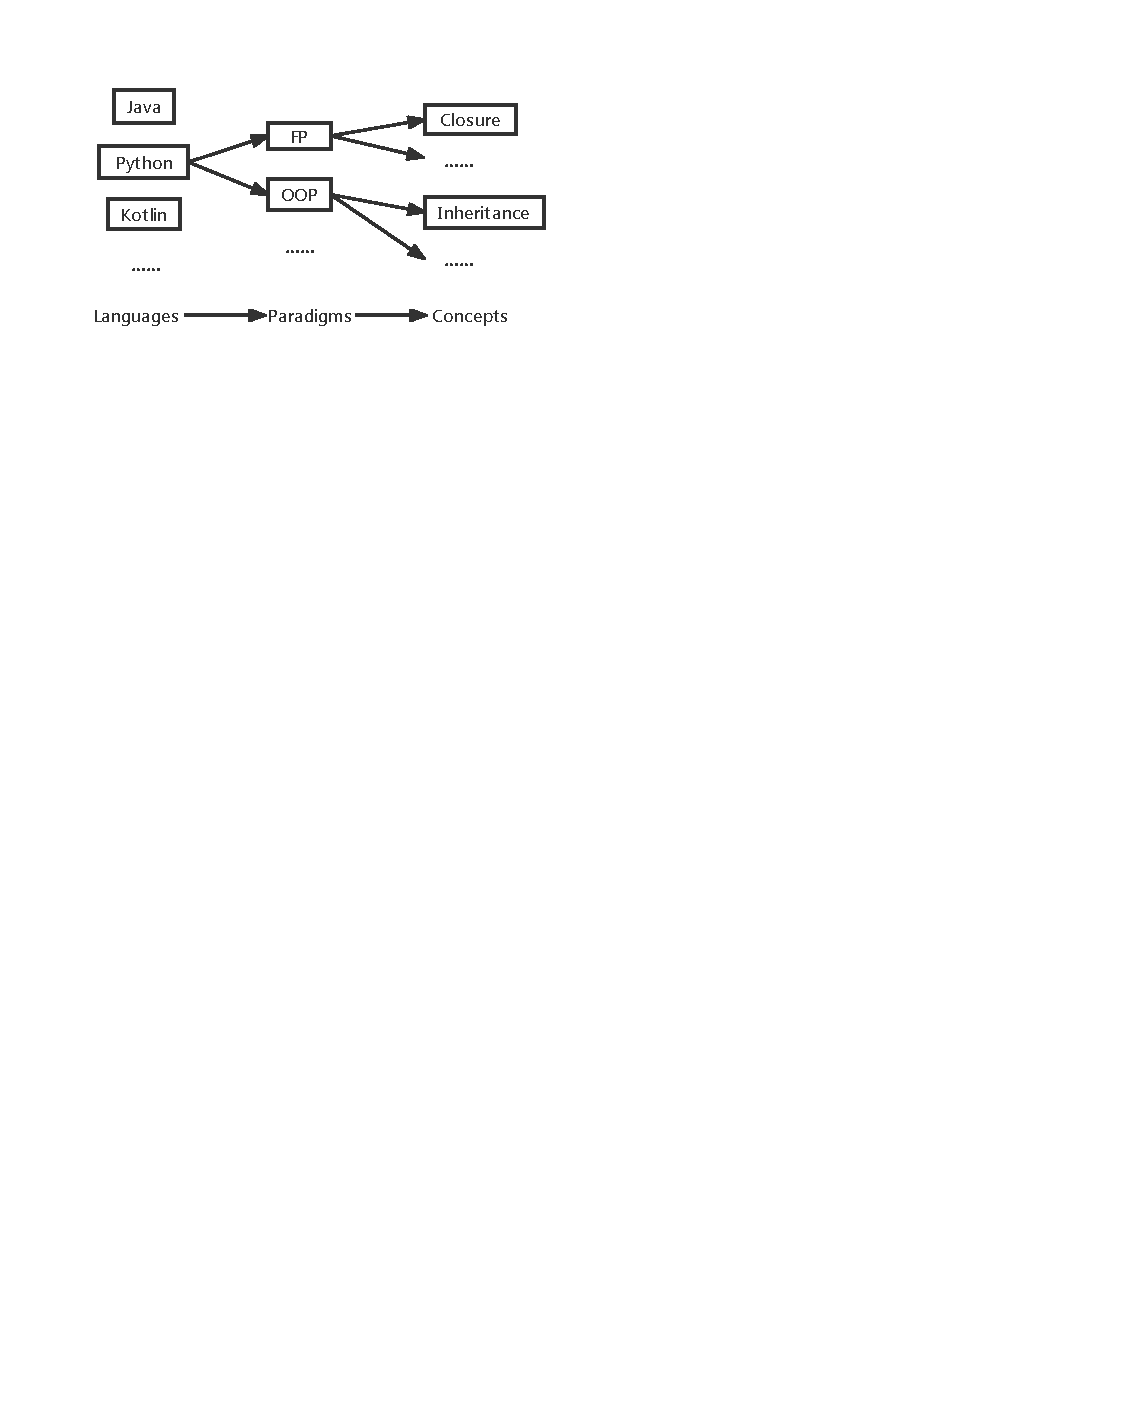
\includegraphics[scale=0.8]{figures/concept}}
    \caption{Languages, paradigms, and concepts}
    \label{fig:concept}
\end{figure}

The figure shows the relationship between languages, paradigms, and concepts. Each paradigm contains a core set of concepts, and each language also realizes one or more paradigms. FP and OOP are programming paradigms that are commonly available in MPLs. However, the degree of support for them varies from one programming language to another. The table shows the degree of support for the concepts of FP and OOP in each language.

For the concepts in the programming paradigm, a more practice-oriented organization is here. It will favor the choice of concepts defined in specific programming languages over those in programming paradigm theory. For example, for the functional concept of nested and anonymous functions, they are implemented as lambda expressions in many programming languages. Again, for example, for the object-oriented concept of combination, most of the currently popular programming languages support it. For programming language design, the combination is simply a way of arranging data. It does not belong to any paradigm. Even languages like the more ancient one, C, provide structure combinations and function combinations. Therefore, combinations are not included in the analysis.

\begin{table*}[htbp]
    \caption{Several concepts of FP and OOP}
    \label{tab:concept}
    \begin{center}
        \begin{tabular}{cll}
            \toprule
            Paradigm & Concept & Meaning \\
            \midrule
            FP & Higher-order function & Take functions as variables, which can
            pass as parameters or return values. \\
            FP & Lambda expression & A short block of code which takes in parameters
            and returns a value. \\
            FP & Partial application & Given a function with certain parameters,
            producing another function (with fewer parameters). \\
            FP & Closure & A record stores a function together with an
            environment\cite{sussman1998scheme}. \\
            FP & Type inference & The automatic detection of the type of an
            expression at compile time. \\
            FP & Pattern matching & Dispatch branch by matching the pattern of a
            given sequence of tokens. \\
            FP & Statement as expression & Take all statements as expressions, which
            creates a definite value. \\
            OOP & Encapsulation & Hide the properties and implementation details of
            the object, and only expose the interface to the outside. \\
            OOP & Inheritance & Create classes that are built upon existing
            classes\cite{johnson1988designing}. A way of
            code reuse. \\
            OOP & Composition & Combine entities into more complex ones. A way of
            code reuse. \\
            OOP & Delegation & One entity passing something to another
            entity\cite{wilkinson2009grid}. A way of code
            reuse. \\
            OOP & Trait & A set of method conventions. Broadly including trait,
            interface, protocol and mixin. \\
            OOP & Polymorphism & Use of a single symbol to represent multiple
            different
            types\cite{cardelli1985understanding}. \\
            OOP & Everything is object & All the basic elements of a programming
            language are represented in the form of objects. \\
            \bottomrule
        \end{tabular}
    \end{center}
\end{table*}

\subsection{Functional programming}

The most important feature of FP is its high degree of abstraction. This is mainly because FP has its origins in the lambda calculus, so it has some of the characteristics of abstract algebra. In the practice of FP, the main idea is the combination and nesting of higher-order functions, so the core of its design is to sort out the rules of nesting and combination of higher-order functions. Thus, the basic design approach can be described as follows. Based on the standardization of the function transfer model and the combinability of higher-order functions, the description of the mapping of data from the source to the result is completed through a series of rule designs. Here the mapping is done by a formal combination of several higher-order functions. Descriptions are like mathematical formulas that map input data into results through layers of iterations. For the iterative process of data in a broad sense, which includes not only the iteration of the data itself, but also the iteration of the rules. This is due to the fact that in functional languages, data and rules are semantically unified in functions.

As programming language practice continues to deepen, programming languages are becoming more and more supportive of functional concepts. For programming languages released in the 1980s and 1990s, the support for functional concepts was not good when they were first created. This is especially true for Java and C++. From the original syntax, one did not design them with FP in mind. And for JavaScript and Python, they are a bit better in this regard. Although they inherently support some functional concepts, they are still missing some advanced functional concepts. As for the programming languages released around 2010, they all support the basic functional concept. In particular, Rust and Kotlin additionally support the concept of "statements as expressions", a milestone in the development of MPL paradigm convergence. The concept of "statements as expressions" is more common in functional languages and provides semantic unification of expressions and statements. However, this concept is not supported in most programming languages with paradigm convergence. As programming languages continue to evolve, Kotlin and Rust are supporting this concept with paradigm convergence. Thus Kotlin and Rust can be considered as having a higher level of support for FP concepts.


\begin{table*}[hb]
    \caption{Degree of support for FP concept}
    \label{tab:fp}
    \begin{center}
        \begin{tabular}{cccccccc}
            \toprule
            Language & Higher-order functions & Lambda expression & Partial
            application & Closures & Type inference & Pattern matching & Statements
            as expressions\\
            \midrule
            Python     & \Checkmark & \Checkmark & Python2.5   & \Checkmark & \Checkmark & Python3.10  & ×          \\
            Java       & Java8      & Java8      & Java8       & Java8      & Java10     & ×           & ×          \\
            C++        & C++11      & C++11      & C++11       & C++11      & C++11      & C++17       & ×          \\
            JavaScript & \Checkmark & \Checkmark & ECMAScript5 & \Checkmark & \Checkmark & ECMAScript6 & ×          \\
            Go         & \Checkmark & \Checkmark & \Checkmark  & \Checkmark & \Checkmark & ×           & ×          \\
            Swift      & \Checkmark & \Checkmark & \Checkmark  & \Checkmark & \Checkmark & \Checkmark  & ×          \\
            Dart       & \Checkmark & \Checkmark & \Checkmark  & \Checkmark & \Checkmark & ×           & ×          \\
            Rust       & \Checkmark & \Checkmark & \Checkmark  & \Checkmark & \Checkmark & \Checkmark  & \Checkmark \\
            Kotlin     & \Checkmark & \Checkmark & \Checkmark  & \Checkmark & \Checkmark & \Checkmark  & \Checkmark \\
            \bottomrule
        \end{tabular}
    \end{center}
\end{table*}

\subsection{Object oriented orogramming}
The most important feature of OOP is its emphasis on reuse. Back in the 1960s, software maintenance became increasingly difficult due to the increasing complexity of hardware and software. OOP solves this problem by emphasizing reusability. In the practice of OOP, one maps real problems into entities and their relationships, rather than being concerned with the process of dealing with the problem. After the birth of object-oriented languages, there was an urgent need to map from problems to entities and relationships in a modeling way, at which point UML was born. It is a set of standardized modeling languages for visualization and has greatly contributed to the development of object-oriented methodologies. Since then the practice of OOP has always emphasized design before implementation.

For the core concepts of OOP, there is not much difference in the level of support of MPLs. Because of its relatively long history and the lack of revolutionary innovations in theory and practice in recent years, most programming languages have implemented the core concepts of OOP relatively completely. In addition, more and more programming languages are realizing object-oriented features by supporting combinations and delegates, while mere inheritance has proven to be bad practice. Therefore, the concept of classes and inheritance is abandoned in Go and Rust, and object orientation is realized through trait. Compared to class-based object-oriented, trait-based object-oriented has a looser coupling and more flexible realization. However, most MPLs support both trait and class for different granularity of control.

In order to more accurately distinguish the degree of OOP concept support for each MPL, some concepts that are not commonly used are introduced here. An example is "everything is object". According to the definition of OOP, it should have been the most basic concept in OOP. In fact, however, early programming languages tended to have a large number of imperative features, i.e., not all elements were treated as objects. For example, there are still primitive data types in Java, which are not objects, so we cannot call methods of these types as if they were objects. Perhaps there are many performance positives of primitive data types, but from a semantic consistency perspective, primitive data types have negative effects. Therefore, languages with the concept of "everything is object" are considered to have a higher level of OOP support.

\begin{table*}[htbp]
    \caption{Degree of support for OOP concept}
    \label{tab:oop}
    \begin{center}
        \begin{tabular}{cccccc}
            \toprule
            Language & Inheritance & Delegation & Traits & Polymorphism &
            Everything is object \\
            \midrule
            Python     & \Checkmark & \Checkmark & ×          & \Checkmark & \Checkmark \\
            Java       & \Checkmark & ×          & \Checkmark & \Checkmark & ×          \\
            C++        & \Checkmark & ×          & \Checkmark & \Checkmark & ×          \\
            JavaScript & \Checkmark & \Checkmark & ×          & \Checkmark & \Checkmark \\
            Go         & ×          & ×          & \Checkmark & \Checkmark & ×          \\
            Swift      & \Checkmark & ×          & \Checkmark & \Checkmark & \Checkmark \\
            Dart       & \Checkmark & ×          & ×          & \Checkmark & \Checkmark \\
            Rust       & ×          & \Checkmark & \Checkmark & \Checkmark & \Checkmark \\
            Kotlin     & \Checkmark & \Checkmark & \Checkmark & \Checkmark & \Checkmark \\
            \bottomrule
        \end{tabular}
    \end{center}
\end{table*}

\subsection{Programming Paradigms and Applications}

\begin{figure}[htbp]
    \centerline{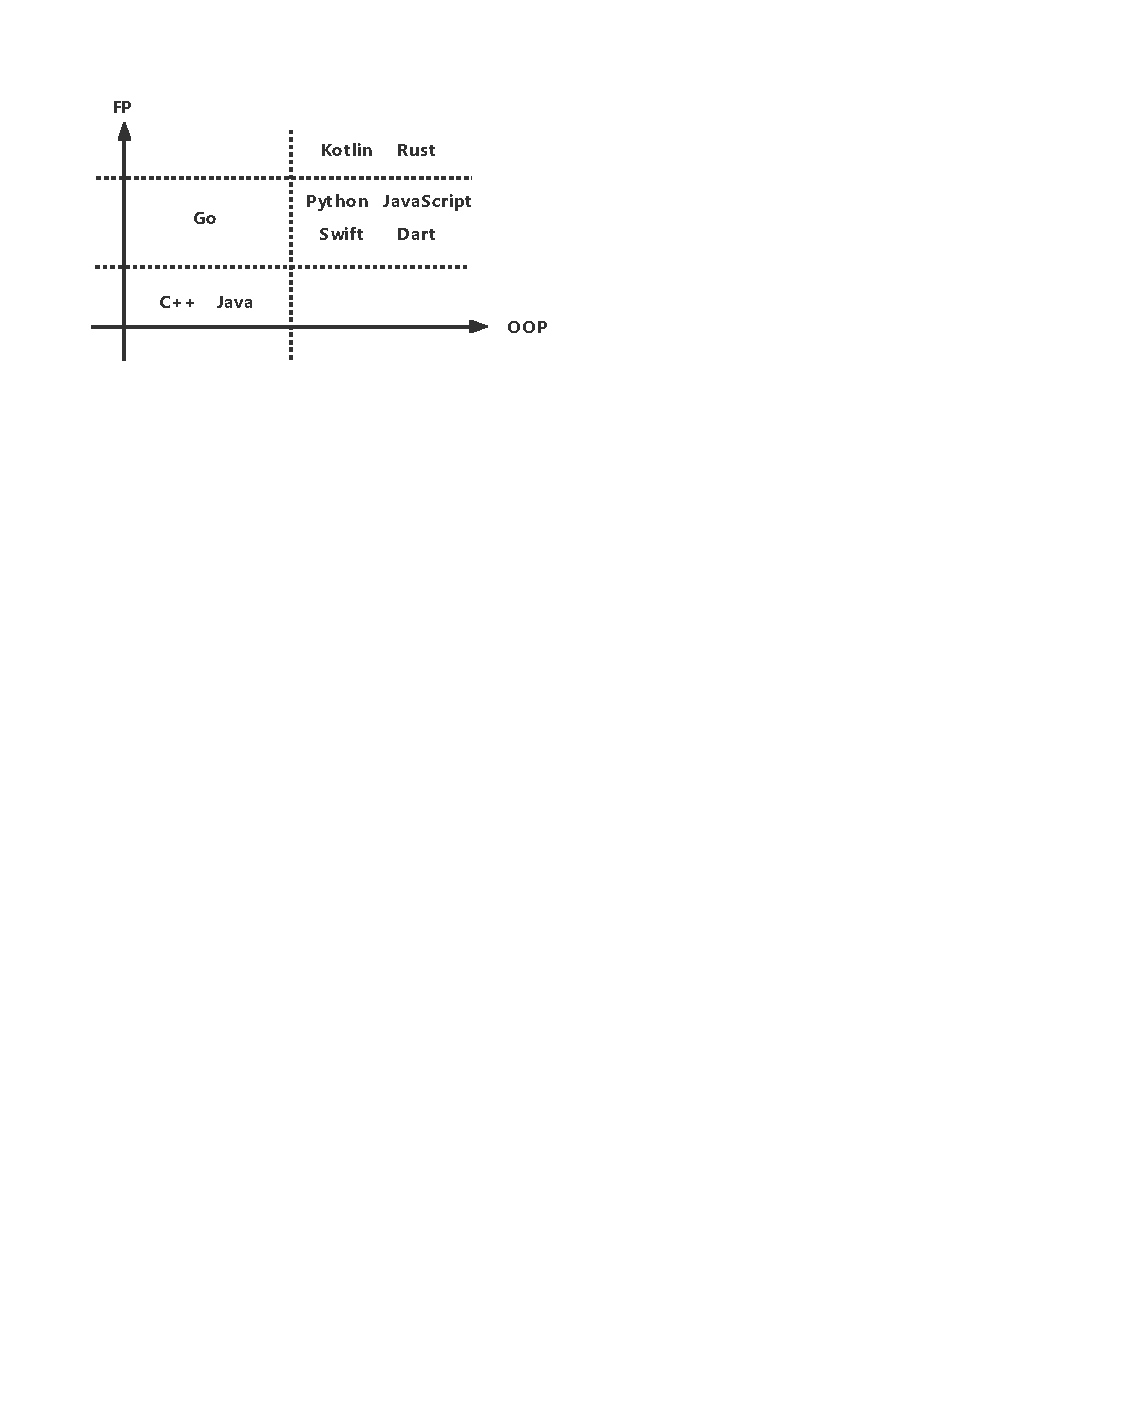
\includegraphics[scale=0.8]{figures/paradigm}}
    \caption{Degree of programming paradigm concept support}
    \label{fig:paradigm}
\end{figure}

The above discussion leads to this diagram, which roughly depicts the degree of support for FP and OOP concepts in different programming languages. For a given programming language, the closer it is to FP/OOP in the figure, the better it supports FP/OOP. In fact, the paradigm of a programming language is very closely related to its application scenario, whether it is for a single application area or for multiple application areas.

A typical example is Dart. Its main application scenario is the Web front-end, and it is often used as a support language for the GUI framework Flutter. It is obvious that most of the GUI frameworks we use have a complex inheritance structure. This is because, for GUIs, most of its application scenarios satisfy the Liskov Substitution Principle, i.e., the child type can completely replace the parent type. This is a sufficient condition for using inheritance. Therefore, Dart only provides object-oriented concepts based on inheritance.

The next example is Java, which has weak support for both FP and OOP concepts. In the early years, Java was used for Enterprise development. Later it was used for Web servers, a scenario that required high abstraction of business logic, so Java added the additional concept of FP. However, due to the design of the language itself, the level of support is not high.

Another example is Kotlin, which has better support for both FP and OOP. Its initial application scenario is Android. In order to solve the previous problem that Java was too cumbersome to develop Android applications, Kotlin was designed to add a lot of FP and OOP concepts for the Android application scenario. Not only does it support traditional FP and OOP concepts, but it also makes syntax-level optimizations for these concepts, such as the FP syntactic sugar "trailing lambda" and the OOP delegate syntactic sugar "by". These useful features in turn allow Kotlin to be used in other scenarios, such as server front-ends and back-ends.